%%   This file is part of the APS files in the REVTeX 4 distribution.
%%   Version 4.0 of REVTeX, August 2001
%%
%%
%%   Copyright (c) 2001 The American Physical Society.
%%
%%   See the REVTeX 4 README file for restrictions and more information.
%%
%
% This is a template for producing manuscripts for use with REVTEX 4.0
% Copy this file to another name and then work on that file.
% That way, you always have this original template file to use.
%
% Group addresses by affiliation; use superscriptaddress for long
% author lists, or if there are many overlapping affiliations.
% For Phys. Rev. appearance, change preprint to twocolumn.
% Choose pra, prb, prc, prd, pre, prl, prstab, or rmp for journal
%  Add 'draft' option to mark overfull boxes with black boxes
%  Add 'showpacs' option to make PACS codes appear

% Edited by Camilla Harris Jan 2015
% For use by Camilla Harris, Akshat Mahajan
% in creating Lab Reports for 180c at UCLA
% this file and auxiliary files were retrieved from
% http://www-d0.fnal.gov/Run2Physics/WWW/templates/
% on Jan 19 2015

\documentclass[aps,prl,nofootinbib,twocolumn,superscriptaddress,groupedaddress]{revtex4}  % for review and submission
%\documentclass[aps,preprint,superscriptaddress,groupedaddress]{revtex4}  % for double-spaced preprint
% CAMILLA: I removed the PACS functionality
\usepackage{graphicx}  % needed for figures
	%if using postscript files compile with XeLaTex
\usepackage{dcolumn}   % needed for some tables
\usepackage{bm}        % for math
\usepackage{amssymb}   % for math
\usepackage[export]{adjustbox}
\usepackage{array}
\usepackage{multirow, bigdelim}

% avoids incorrect hyphenation, added Nov/08 by SSR
\hyphenation{ALPGEN}
\hyphenation{EVTGEN}
\hyphenation{PYTHIA}

\begin{document}
\title{Experiments with Pulsed Nuclear Magnetic Resonance}
\input author_list.tex        % includes institutions and visitors
\date{\today}

\begin{abstract}
In this paper, we explore aspects of pulse-burst nuclear magnetic resonance with capsules of water of varying purity. Exposing our samples to fixed-magnitude discrete `bursts' of sinusoidally varying magnetic field components in the $x,y$-plane while in the presence of a static magnetic magnetic field oriented in the $z$ direction, we attempted to measure the spin lattice relaxation-time $T_{1}$ as well as the phase decoherence time $T_{2}$ with appropriate pulse lengths. A linear trend for $\frac{1}{T_{1}}$ with varying magnetic impurity levels was found.
\end{abstract}

\maketitle

\section{Background Information}
Pulsed nuclear magnetic resonance (NMR) refers to the production of a radio-frequency wave from an atomic nuclei following interaction with short-lived external radio-frequency waves of appropriate frequency in directions transverse to a static, essentially spatially homogeneous magnetic field component perpendicular to the direction of the waves. More precisely, application of the field \begin{equation}
\vec{B}(x,y,z,t) = B_{1}\cos \omega t \hat{x} + B_{1}\sin \omega t \hat{y} + B_{0}\hat{z}
\end{equation}
to a population of random, unoriented nuclei with associated magnetic moment for short times leads to the production of a measurable radio-frequency signal from these nuclei - this constitutes pulsed NMR\cite{lab}.

Spin polarization, whereby a sample of particles with randomly aligned spins resolves itself into two sub-populations with spins either aligned or anti-aligned along a particular direction respectively, takes place in the presence of an external uniform magnetic field $B_{0}\hat{z}$. These sub-populations differ in energy by amount $2\mu_{B}B$, where $\mu_{B}$ is the Bohr magneton with value 9.27 $\times 10^{-24}$ J T$^{-1}$. Populations with anti-parallel spin $-\frac{1}{2}$ have higher energy, and each subpopulation has corresponding magnetic moment $M(\pm z)$ - the positive sign refers to the magnetic moment in the positive direction for the population with positive sign, and the negative sign in the negative direction for the population with negative spin.

Given time, the spin distribution begins to collapse into a thermal equilibrium distribution (with associated equilibrium moment $M_{0}$), as spins with higher energy relax to a state with lower energy. This relaxation takes place on a characteristic timescale $T_{1}$. In particular, the proportion of the population $N_{z}$ aligned parallel to the field grows towards a thermal equilibrium state $N_{0}$ thanks to the additive effect of higher-energy spins relaxing into the parallel spin state. The corresponding equation for the magnetic moment of the positive spin population is given by\cite{inst} (for C = 1)
\begin{equation}
M_{z} = M_{o}\left(1 - Ce^{-\frac{t}{T_{1}}}\right)
\end{equation}
\vspace{\baselineskip}
In pulsed NMR, this state of affairs is somewhat modified. Application of the $x$,$y$ components of Eq. 1 for a sufficient period of time in the presence of $B_{0}\hat{z}$ is enough to force the net magnetic moment to precess about the $x$-axis with a frequency of $42.58\cdot B_{0}$ MHz\cite{inst}. A pulse that exists for a precisely calibrated period of time is sufficient to `flip' the magnetic moment completely along the $-z$ plane (in other words, spin is flipped by 180$^{\circ}$ along the $x$-axis). Measurements of the decay parameter $T_{1}$ (also called the \textsl{spin relaxation time}) can be made from the radio-frequency signal produced by the nuclei as they relax back into states aligned with the $z$ axis. Eq. 2 can be used to describe this case\cite{inst} with C = 2.

Another important decay phenomenon occurs when the $x,y$ component forces a magnetic moment entirely in the $x,y$ plane that is distinctly non-equilibrium (in other words, magnetization is first flipped to align in the $x,y$ plane before being flipped 180$^{\circ}$ within the $x,y$ plane following a certain delay time). Given time, this non-equilibrium distribution is lost due to thermal irreversible processes, forcing the individual moments to start to diverge in the $x,y$ plane on a timescale $T_{2}$. This parameter is called the \textsl{spin-spin relaxation time}, and can be thought of as the \textsl{phase decoherence time}. Measurement of $T_{2}$ is accomplished by measuring the height of the spin echo - an alignment of the $x,y$ plane magnetization in the opposite direction as the original magnetization due to the diverging individual magnetic moments aligns briefly in the opposite direction - versus delay time (see Experiment Details). 

Finally, we note that magnetic impurities have an effect on the timescale $T_{1}$. In particular, magnetic impurities tend to have both electronic and nuclear magnetic moment more tightly coupled than in non-magnetic samples. Consequently, we find that\cite{lab} 
\begin{equation}
\textrm{impurity amount} \propto \frac{1}{T_{1}}
\end{equation}

\section{Experiment Details}

\begin{figure}[t]
\centering
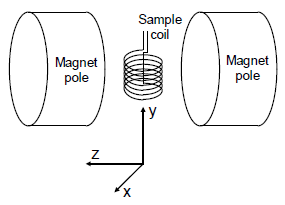
\includegraphics[scale = 0.6]{instrument.PNG}
\caption{Sketch of basic experimental setup. Image sourced from \cite{inst}} 
\end{figure}

\begin{figure}[t]
\centering
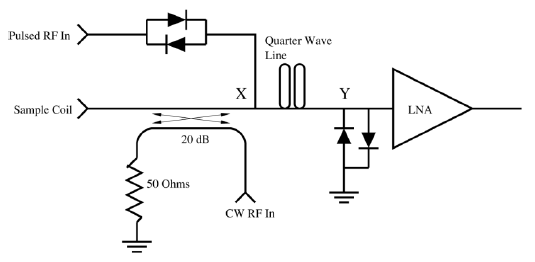
\includegraphics[scale = 0.6]{schematic.PNG}
\caption{Experimental schematic. Image sourced from \cite{inst}} 
\end{figure}

For our pulsed NMR experiments, a Pulsed/CW NMR TeachSpin spectrometer model PS2 was used. Samples of water of varying concentration of impurities (pure, 0.3125 M impure, 0.625 M impure, 1.25 M impure and 2.5 M impure respectively) were placed in a sample coil exposed to a lateral homogeneous magnetic field of amplitude 0.5 $\pm$ 0.02 Tesla (see Fig. 1). The sample coil is able to pick up $EMF$ variations within the $x,y$-plane, and this information is passed to the spectrometer. The spectrometer never measures $M_{z}$ directly, but instead can only precession in the $x,y$ plane. The spectrometer also has two channels for measurement, where the second channel is essentially the first channel with a phase difference of $\pi/2$. A lock-in amplifier phase-separates signals into two separate channels, where the second channel is essentially the first channel with a phase difference of $\pi/2$.

Calibration of the angular frequency of the wave is necessary prior to application of the $x,y$ components. Successful `flipping' purely about the $x$-axis occurs when the frequency of the wave is matched perfectly with the precession frequency of the nuclei; however, the precession frequency is not necessarily known prior to experiment, so it is important to identify it prior to any other experiment. This calibration was accomplished by a single-pulse measurement, whereby the frequency and duration of a pulse A was varied so as to result in maximum signal from the nuclei. Only maximum magnetization within the $x,y$ plane (a 90$^{\circ}$ flip) at the precession frequency of the nuclei results in maximum signal - thus, we were able to precisely calibrate our instrument this way.

In order to ensure improved accuracy of $T_{1}$, the TeachSpin apparatus employs a two-pulse tactic, whereby two magnetic pulses A and B, with different lengths, are used to control the spins in a manner that maximises the EMF detected from the nuclei. First, a pulse A of suitable length is applied to flip the spins by a complete 180$^{\circ}$, following which a pulse B of half that length orients all spins so that they lie within the $x,y$ plane. The resulting signal is proportional to $M_{z}$ just before application of B, so that we can measure the strength of $M_{z}$ indirectly. The application of B after A is delayed by a certain period of time each run so as to construct a time-dependence graph of $M_{z}$; this time delay is within our control, and the experiment was conducted with different values of the time delay. Visual inspection of raw data was done to obtain the calibration frequency. Our calibration frequency was 21.45970 MHz, which is slightly higher than the accepted value of 21.29 MHz derived by application of the formula $42.58\cdot B_{0}$.

In order to ensure improved accuracy of $T_{2}$, the TeachSpin apparatus employs a two-pulse tactic, whereby magnetic pulses A and B are used to control the spins in a manner that maximises the EMF detected from the nuclei. A pulse A of suitable length is applied to flip the magnetic moment by a complete 90$^{\circ}$, following which pulse B flips the magnetic moment by 180$^{\circ}$. In other words, the signal lengths are the reverse of those used to determine $T_{1}$. Signals along the $x,y$ plane are measured. It is important to note that, while phase decoherence is occuring, relaxation back into a $z$-aligned state is \textit{also} occuring - however, the orientation of our spectrometer prevents detection of this second phenomenon, so we only get a pure signal regarding phase decoherence in the $x,y$ plane. The application of B after A is delayed by a certain period of time each run so as to construct a time-dependence graph of the height of the spin echo; this time delay is within our control, and the experiment was conducted with different values of the time delay. The behaviour is roughly given for the magnetization $M_{x}$ in the $x,y$ plane by\cite{inst}
\begin{equation}
M_{x} = M_{0}e^{-\frac{t}{T_{2}}}
\end{equation}

Finally, measurement of $T_{1}$ was repeated with samples of different impurities. The variation of $T_{1}$ with sample impurities can be measured to produce a final rate of change with impurity. 

\section{Results}

The results of our calibration data can be seen in Fig. 3. Our chosen frequency was 21.45970 MHz, obtained by visual inspection. The duration of the pulse length was incremented by 100 ms from 0.06 ms (lowest length setting possible) for fourteen successive turns, so that the pulse length varied from 0.06 ms to 1.46 ms, whereupon the data was seen to have executed a full sine curve. For Channel 1 data, the data was extracted from the maxima immediately prior to the decay of the signal; for Channel 2 data, which is Channel 1 data with a phase shaft of 90$^{\circ}$, the corresponding minima was chosen. Both datasets were obtained using MATLAB's point-picker tool, which enables visual inspection of the data with precise information about each point. Both sets of data were assigned an initial value of 0 for 0.06 ms as the signal was not visible at that pulse length. Estimates for calibrated pulse duration can be found in Table I.

\begin{figure}[t]
\centering
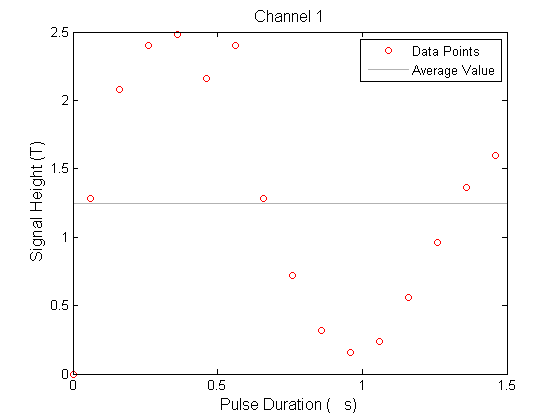
\includegraphics[width=0.5\textwidth]{../Analysis/calibration_channel_1.png} 
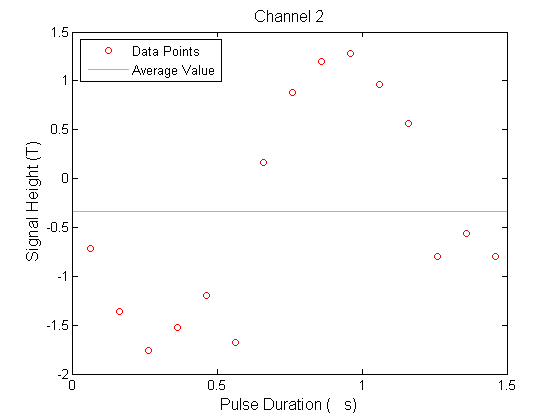
\includegraphics[width=0.5\textwidth]{../Analysis/calibration_channel_2.png}
\caption{Nuclei response signal for various pulse length durations. The roughly sinusoidal variation allows us to calibrate our pulse lengths as to produce a deflection in magnetic moment by at least 90$^{\circ}$}.
\end{figure}

\begin{figure}[t]
\centering
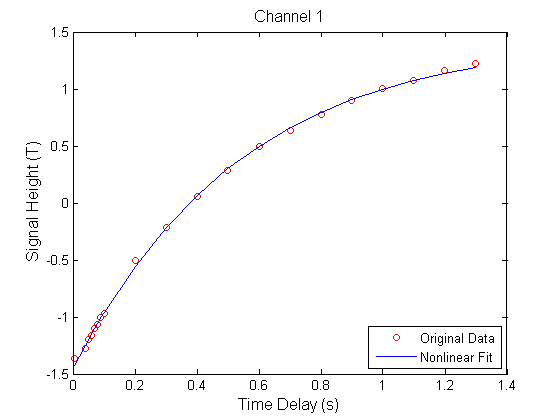
\includegraphics[width=0.5\textwidth]{../Analysis/T1.png} 
\caption{$T_{1}$ measurement data. Signal response vs. time lag between A and B pulses clearly shows an exponential rising trend. The nonlinear fit is performed with Eq. 2 for $C = 2$, with $M_{0}$, $T_{1}$ as parameters; they  were found to be 1.59 T and 0.53 s respectively} 
\end{figure}

\begin{figure}[b]
\centering
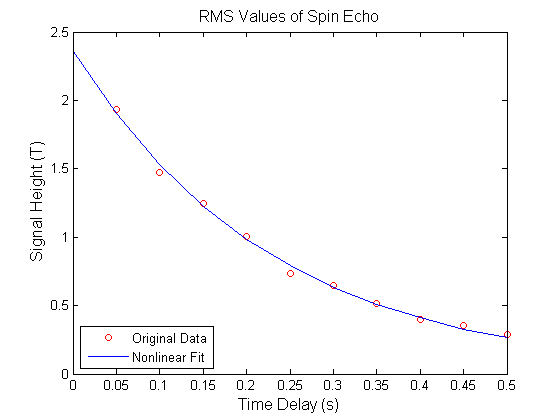
\includegraphics[width=0.5\textwidth]{../Analysis/T2.png} 
\caption{$T_{2}$ measurement data. Signal response vs. time lag between A and B pulses clearly shows an exponential decreasing trend. The nonlinear fit is performed with Eq. 4 with $M_{0}$, $T_{2}$ as parameters; they  were found to be 2.37 T and 0.22 s respectively} 
\end{figure}

For $T_{1}$ measurements, a different approach was used to obtain the data points. Instead of visually picking points, the global maximum was first chosen. The average of the next 100 points was taken, with the knowledge that the oscillatory component of the signal would cancel out the bias involved with the maximum and provide an estimated average value. This method was chosen in order to overcome the difficulties involved with distinguishing maxima/minima visually in the data. Errors associated with this method are discussed in the Analysis section. Fig. 4. displays the results of our investigation into $T_{1}$, with a nonlinear fit corresponding to Eq. 2 with $C = 2$. Both $M_{0}$ and $T_{1}$ were parameters in our nonlinear fit, and were found to be 1.59 T and 0.53 s respectively, computed via MATLAB's nonlinear fit iterative algorithm. Different seed values, varying from 1 to 25 for each parameter for this algorithm were chosen, and were found to converge to these values regardless, indicating an independence of seed value and a potentially robust fit. An analysis of the potential error of this fit is presented in the Analysis section.

For $T_{2}$ measurements, determining the height of the spin echo is paramount. However, because of phase decoherence, there is a phase component involved in Channel 1 and Channel 2 that must not be neglected. Therefore, an accurate estimation of the spin echo value comes by taking the root mean square of the spin echo heights. In other words, we take the square root of the sum of squares of the corresponding spin echo height from channels 1 and 2. This procedure was not applied elsewhere as no other part of the experiment depended explicitly on phase component.

Finally, we attempted to obtain a dependence of $T_{1}$ on the impurities involved, using the same algorithm by which points for $T_{1}$ were obtained in Fig 4. Figure 6 showcases our results. We obtained measures for $T_{1}$ by using MATLAB's \texttt{nlinfit} function. Our final estimates regarding $T_{1}$ estimates as a function of concentration is presented in Table II.

\onecolumngrid

\begin{figure}[b]
\centering
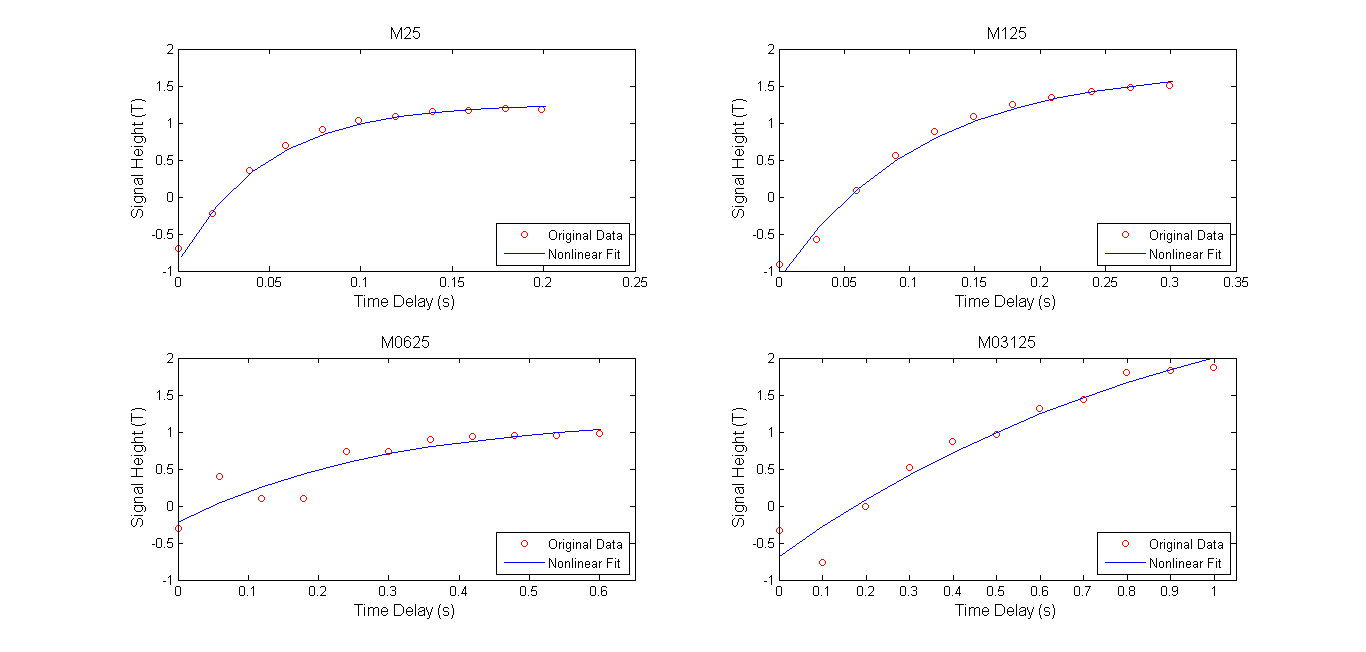
\includegraphics[width = \textwidth]{../Analysis/impurity.png}
\caption{Our measurements of $T_{1}$ for different molar concentrations, indicated in the title via a simple code e.g. M25 corresponds to 0.25 M of solute within our liquid solution. Offsets were included as a parameter in the nonlinear fit to compensate for non-zero values of the data at or close to the origin.}
\end{figure}

\twocolumngrid
\begin{table}[t]
\caption{Calibration pulse durations at 90$^{\circ}$ derived from various `angles' in the sinusoidally-varying data in Fig. 3. For example, the pulse value of an angle at 270$^{\circ}$ (the minimum) is divided by 3 to get the corresponding value at 90$^{\circ}$. All pulse values are in seconds. See Analysis section for description of our procedure.}
\begin{ruledtabular}
\begin{tabular}{ccp{18mm}ccp{18 mm}}
Angle & Pulse & Pulse at 90$^{\circ}$ (Channel 1) & Angle & Pulse & Pulse at 90$^{\circ}$ (Channel 2)\\
\hline
90$^{\circ}$ & 0.36 & 0.36 & 90$^{\circ}$ & 0.26 & 0.26 \\
180$^{\circ}$ & 0.66 & 0.36 & 180$^{\circ}$ & 0.56 & 0.28 \\
270$^{\circ}$ & 0.96 & 0.36 & 360$^{\circ}$ & 0.96 & 0.36 \\
360$^{\circ}$ & 1.36 & 0.34 & 360$^{\circ}$ & 1.36 & 0.34 \\
\hline
\multicolumn{6}{c}{Average Value at 90$^{\circ}$ (All Channels)}\\
\multicolumn{6}{c}{0.3325 $\pm$ 0.0399 s}
\end{tabular}
\end{ruledtabular}
\end{table}
\
\section{Analysis}

One possible source of systematic error that has the potential to affect all other measurements may be our slightly high value of precession frequency 21.49 MHz. A higher value of precession frequency than needed for the energy difference between the spin-up and spin-down oriented states can lead to a lower percentage of  spin-up states transferring to the spin-down states. For $T_{1}$ measurements, this means that it will not take as much time for the net magnetization to return to thermal equilibrium, leading to an underestimation of $T_{1}$. However, the theoretical value and our chosen value differ by only 1\% with respect to 21.29 MHz, meaning that the error that accrues owing to this is small enough to be negligible. This is not therefore a serious source of systematic error. 

We outline, as follows, our procedure for estimating the pulse duration for which a deflection of magnetisation by 90$^{\circ}$ is observed (in other words, how we arrive at our calibration). Given that a clear sinusoidal variation is observed in Channel 1, we estimate the deflection by 90$^{\circ}$ to occur at the first maximum, a deflection by 180$^{\circ}$ to occur at the value closest to zero after the first maximum, a deflection by 270$^{\circ}$ to occur at the first minimum and a deflection by 360$^{\circ}$ to occur at the value closest to zero after the first minimum. From each of these values, we are able to reconstruct the value at 90$^{\circ}$ by simply dividing the value by the multiple of 90 degrees to which the angle corresponds. For Channel 2, which differs from Channel 1 by a phase difference of $\pi/2$, these estimations are shifted accordingly. Table I presents our data, and an example of our procedure is provided in the adjoined caption. We arrive at an estimate of 0.3325 $\pm$ 0.0399 s as the appropriate pulse duration to produce deflection by 90$^{\circ}$.

We now analyse our $T_{1}$ measurements. One important source of systematic error in this regard may stem from our method of selecting for these values - in particular, our algorithm depends heavily on large oscillations after the maximum cancelling out evenly and producing an overall average that is representative of the amplitude of the response from our nuclei. These oscillations (so-called free inductive decay) arise from the inductive effects due to the generation of magnetic moment as spins rapidly align, and our chief interest lies in the amplitude of the response immediately prior to its decay to near-zero values (i.e. when the magnetic field is turned off). However, it is always possible that our oscillations did not cancel out evenly, and thus that we are over- or under-estimating our values.

We test this hypothesis by collecting data instead by taking the \textit{median} of the values after the maximum instead. As a central measure of tendency, the median is significantly less affected by extremes than the mean - if the oscillations do not cancel out evenly, there should be a significant discrepancy between the values obtained by these two methods. Fig. 7 depicts the differences between both collection techniques. From a cursory examination of our results, it becomes immediately clear that no significant differences between these two collection methods are apparent - both collection techniques find the same value, with \textit{no} values differing from each other. We therefore argue that the oscillations do in fact cancel out evenly; however, we caution that this may be a function of window size (i.e. the number of points sampled after the maximum) although no such trend was noticed in this dataset, and more rigorous testing is needed to be done to ensure such consistency in the future.

\begin{figure}[b]
\centering
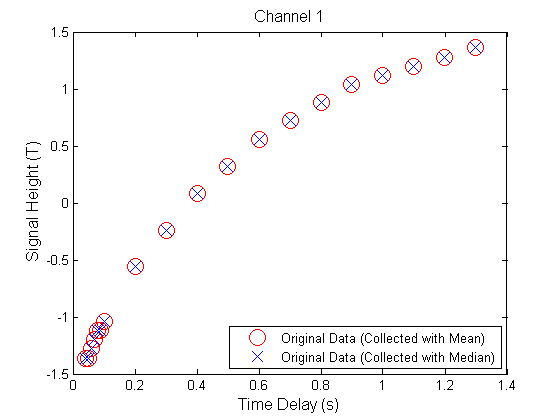
\includegraphics[width=0.5\textwidth]{../Analysis/T1analysis.png} 
\caption{Collecting $T_{1}$ data with the mean versus collecting it with the median. Marker sizes are larger than those in Fig. 4 for improved visibility. The data point at the origin was omitted for clarity of presentation, but is otherwise unchanged, and also demonstrates the same behaviour as the rest of the points do with both methods.} 
\end{figure}

Another source of systematic error could stem from our nonlinear fit. We report a mean standard error (MSE) of about 0.010 for our fit, indicating a degree-of-freedom corrected $R^{2}$ regression coefficient value in excess of 90\%. Evaluating the goodness of fit of a nonlinear model is complicated, and we advise not to take the $R^{2}$ regression coefficient value at face value. We currently know of no other way to evaluate nonlinear regression fitting.

Finally, one important source of systematic error that must not be ignored may be a lack of sufficient time between successive measurements. The $T_{1}$ measurements can only be sensibly interpreted if sufficient time is allowed after every measurement to let the system reach the thermal equilibrium distribution - otherwise, repeating the measurement part way through the relaxation results in a disturbance of a non-equilibrium thermal distribution of magnetisation, which in turn provides a false reading. Between every measurement, at most five seconds elapsed. Ideally, the gap between each measurement should be much, much longer than the spin relaxation time, and, while we feel justified about our time gap between measurements following our non-linear fit, a much longer time gap between measurements might have been advisable.

We now discuss sources of error for our $T_{2}$ measurement. Our nonlinear fits for $T_{1}$ and $T_{2}$ disagree with respect to their value for $M_{0}$, indicating a constant offset from our standard value not accounted for in our analysis thus far. This offset could potentially be accounted for by the presence of inhomogeneity in the applied magnetic field, which serves to alter the direction of the net magnetisation. This represents a systematic error that utmost care was taken to prevent, but nevertheless may have occurred. Our mean standard error for $T_{2}$ is 0.011, representing again an $R^{2}$ value in excess of 90\%. 

Sources of random error can include temperature differentials across the surface of the water (which serve to alter the net magnetisation of the material), and lack of shielding from Earth's magnetic field. All care was taken to minimise these random errors - temperature was kept at steady room temperature throughout, and Earth's magnetic field is about six orders of magnitude smaller than our applied magnetic field.

\begin{figure}[t]
\centering
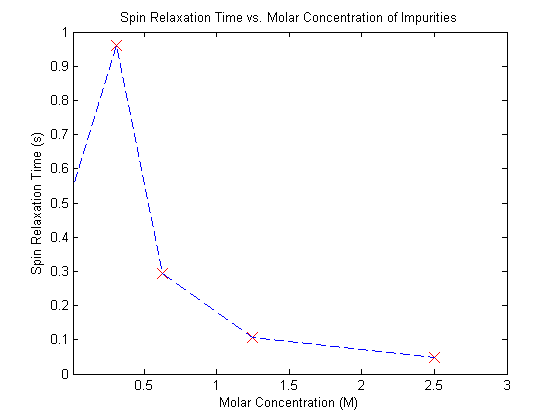
\includegraphics[width=0.5\textwidth]{../Analysis/T1impurity.png} 
\caption{$T_{1}$ vs. molar concentration of impurity. The blue dashed lines connect the red crosses, which represent our data points.} 
\end{figure}

\begin{figure}[t]
\centering
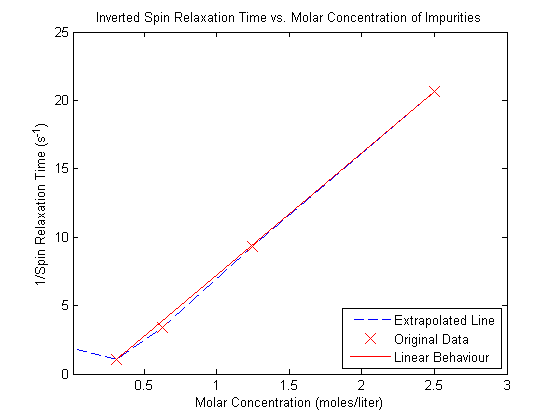
\includegraphics[width=0.5\textwidth]{../Analysis/T1impurity2.png} 
\caption{$\frac{1}{T_{1}}$ versus molar concentration. The red curve indicates the corresponding expected linear behaviour from a concentration of 0.03125 mol/L to 2.5 nols/L, whereas the blue line indicates the actual behaviour. The closeness of these lines indicates agreement.} 
\end{figure}

\begin{table}[b]
\caption{Details of nonlinear fits as described in Fig. 6. Molar concentration refers to the concentration of solute in units of moles/liter (M). MSE stands for Mean Square Error.}
\begin{ruledtabular}
\begin{tabular}{ccccc}
Molar Concentration & $M_{0}$ & $T_{1}$ & Offset & MSE\\
0 & 1.59 & 0.53 & 0 & 0.01\\
0.3125 & 2.08 & 0.96 & 1.39 & 0.05\\
0.625 & 0.71 & 0.29 & 0.50 & 0.03\\
1.25 & 1.40 & 0.10 & 0.32 & 0.008\\
1.25 & 1.05 & 0.04 & 0.20 & 0.001\\
\end{tabular}
\end{ruledtabular}
\end{table}

Finally, we analyse our impurities. In order to arrive at an appropriate value, we were required to add as a parameter a constant offset value to correct for the anomalous value of $M_{0}$, which our analysis of $T_{1}$ and $T_{2}$ also disagree on. The resulting value for the constant offset adjusts the intercept of the fit, but plays a much more marginal role in the slope of the curve. Hence we feel justified in making use of this constant slope value. Table II contains all of the relevant data. We plot a graph of $T_{1}$ versus molar concentration of solute in Fig. 9, and a graph of $1/T_{1}$ versus molar concentration of solute in Fig. 8.

Our results seem to imply that the concentration of impurities is related to the inverse of the magnetic impurities, and is in line with Eq. 3. Despite the strong support with established theory, there is still some cause for concern. In particular, measurements for molar concentrations of 0.3125 M and 0.625 M have the largest associated MSE value, and visually carry some of the worst fits. Further, the behaviour of absolutely pure water is in marked contrast with the behaviour of impure water, for reasons we do not understand. One important cause of this may be a lack of sufficient time between successive measurements - while care was taken to ensure that sampling was not too rapid, it is always possible that the true spin relaxation time was lost because of this. Repeating this experiment may be advisable. At the very least, however, we have demonstrated that impurities do, in fact, have an impact on the spin relaxation time, and that this impact varies linearly with impurity concentrations.

The fact that relaxation rates are dependent on the local environment, however, allows for improved spectroscopic imaging techniques. In particular, it allows for analysis of the composition of materials - comparison with NMR spectra of a pure sample allows for estimation of the quantity of contaminating components. 

\section{Conclusion}
In this experiment, we managed to accurately measure the spin relaxation time and the phase decoherence time for pure (distilled) water. Attempting to measure the spin relaxation time for impure water resulted in a linear dependence, but does not account for the anomalous behaviour of pure water (which, theoretically, should have demonstrated the largest value of $T_{1}$). The sources of error that cause this discrepancy are currently unknown and repeat measurements may need to be made to assess them.

\begin{thebibliography}{2}

\bibitem{lab}
    \textit{Quantum Hall Effect}, Stuart Brown, Physics 180C lab manual of UCLA.
    
\bibitem{inst}
	\textit{Pulsed/CW NMR Spectrometer PS2 - A/B/C Instructor's Manual}, TeachSpin Inc.

\end{thebibliography}

\end{document}